% Build: latexmk (settings in .latexmkrc; the PDF is build/main.pdf). Appearance is in preamble.tex. Figures:
% ../analysis/paper_figures.py and ../analysis/stability_figure.py --partial (data), figures/src/method.tex (diagram).
\documentclass[11pt, a4paper]{article}
% Appearance only; main.tex holds the structure and the text. A single-column technical report in the manner of Moonshot AI's.

% Fonts: STIX Two for text and mathematics, Inconsolata for code and URLs.
\usepackage[T1]{fontenc}
\usepackage{amsmath, amssymb, mathtools}
\usepackage{stix2}
\usepackage[varqu, varl, scaled=0.95]{inconsolata}
\usepackage[english]{babel}
\usepackage{microtype}
\frenchspacing

% Page: A4, 15.5 cm text block, running head in the top margin, page number in the foot.
\usepackage[a4paper, hmargin=2.75cm, vmargin=3cm, headheight=30pt, headsep=0.75cm, footskip=1.2cm, heightrounded]{geometry}

% Paragraphs: separated by half a line, not indented, no widows or orphans.
\setlength{\parindent}{0pt}
\setlength{\parskip}{0.5\baselineskip plus 1pt} % chktex 1
\clubpenalty=10000
\widowpenalty=10000
\displaywidowpenalty=10000
\usepackage{enumitem}
\setlist{itemsep=2pt, parsep=0pt, topsep=0pt}
\renewcommand{\topfraction}{0.85}
\renewcommand{\bottomfraction}{0.7}
\renewcommand{\textfraction}{0.15}
\renewcommand{\floatpagefraction}{0.7}

% Colours: one accent for every link, a grey for the running head and page number.
\usepackage{xcolor}
\definecolor{accent}{rgb}{0.09, 0.5, 0.99}
\colorlet{quiet}{black!55}

% Display equations: the same space above and below.
\makeatletter
\g@addto@macro\normalsize{%
  \setlength{\abovedisplayskip}{10pt plus 2pt}%
  \setlength{\belowdisplayskip}{10pt plus 2pt}%
  \setlength{\abovedisplayshortskip}{\abovedisplayskip}%
  \setlength{\belowdisplayshortskip}{\belowdisplayskip}%
}
\makeatother

% Headings: bold, told apart by size, numbered without a period; \paragraph is a bold run-in heading.
\usepackage{titlesec}
\titleformat{\section}{\normalfont\Large\bfseries}{\thesection}{1em}{}
\titleformat{\subsection}{\normalfont\large\bfseries}{\thesubsection}{1em}{}
\titleformat{\subsubsection}{\normalfont\normalsize\bfseries}{\thesubsubsection}{1em}{}
\titleformat{\paragraph}[runin]{\normalfont\normalsize\bfseries}{}{0pt}{}
\titlespacing*{\section}{0pt}{24pt plus 4pt minus 2pt}{9pt plus 1pt}
\titlespacing*{\subsection}{0pt}{17pt plus 3pt minus 2pt}{5pt plus 1pt}
\titlespacing*{\subsubsection}{0pt}{13pt plus 2pt minus 2pt}{3pt plus 1pt}
\titlespacing*{\paragraph}{0pt}{4pt plus 2pt}{0.6em}

% Every section starts on a new page. The appendix opens with an "Appendix" heading, and its first section follows on the same page.
\newcommand{\sectionpage}{\clearpage}
\AddToHook{cmd/section/before}{\sectionpage}
\AddToHook{cmd/appendix/after}{\clearpage{\LARGE\bfseries Appendix\par}\gdef\sectionpage{\gdef\sectionpage{\clearpage}}}

% Running head (title left, current section right) and page number, small and grey. The first page has the head note above a rule instead.
\usepackage{fancyhdr}
\makeatletter
\newcommand{\subtitle}[1]{\def\@subtitle{#1}}
\newcommand{\headnote}[1]{\def\@headnote{#1}}
\newcommand{\contact}[1]{\def\@contact{#1}}
\subtitle{}
\headnote{}
\contact{}
\pagestyle{fancy}
\fancyhf{}
\renewcommand{\headrulewidth}{0pt}
\fancyhead[L]{\small\itshape\color{quiet}\@title} % chktex 6
\fancyhead[R]{\small\color{quiet}\nouppercase{\leftmark}}
\fancyfoot[C]{\small\color{quiet}\thepage}
\renewcommand{\sectionmark}[1]{\markboth{\thesection\quad #1}{}}
\fancypagestyle{first}{%
  \fancyhf{}%
  \fancyhead[L]{\small\@headnote}%
  \renewcommand{\headrulewidth}{0.5bp}%
  \renewcommand{\headrule}{{\color{black!40}\hrule height \headrulewidth width \headwidth}}% chktex 1
}
\makeatother

% Contents: sections and subsections; entries are links but stay black.
\setcounter{tocdepth}{2}
\AddToHook{cmd/tableofcontents/before}{\begingroup\setlength{\parskip}{0.3\baselineskip}\hypersetup{linkcolor=black}}
\AddToHook{cmd/tableofcontents/after}{\endgroup}

% Figures and tables: "Figure 1: Text", bold label, small text; caption above a table, below a figure. Figures live in figures/.
\usepackage{graphicx}
\graphicspath{{figures/}}
\usepackage{booktabs}
\usepackage{caption}
\usepackage{subcaption}
\captionsetup{font=small, labelfont=bf, labelsep=colon, skip=8pt}
\captionsetup[table]{position=top}
\captionsetup[sub]{font=footnotesize, labelfont=bf}
\renewcommand{\arraystretch}{1.15}

% Footnotes hang from their number.
\usepackage[hang, flushmargin]{footmisc}
\setlength{\footnotemargin}{0.8em}

% Bibliography: numbered, sorted and compressed citations ("[12, 15-17]"), abbrvnat list in \small.
\usepackage[numbers, sort&compress]{natbib}
\bibliographystyle{abbrvnat}
\renewcommand{\bibfont}{\small}
\setlength{\bibsep}{0.35\baselineskip}
\newcommand{\doi}[1]{\href{https://doi.org/#1}{doi:#1}}

% Links: no boxes, all in the accent colour; numbered PDF bookmarks and metadata from the title block.
% \cref writes "Figure 3", "Table 2", "Eq. (4)", "Appendix A", "§2.1"; \Cref, at the start of a sentence, "Equation (4)", "Section 2.1".
\usepackage[bookmarksnumbered, bookmarksopen, bookmarksdepth=3]{hyperref}
\hypersetup{colorlinks=true, allcolors=accent}
\pdfstringdefDisableCommands{\def\\{}}
\makeatletter
\AtBeginDocument{\hypersetup{pdftitle={\@title\ifx\@subtitle\@empty\else: \@subtitle\fi}, pdfauthor={\@author}}}
\makeatother
\usepackage[capitalise, noabbrev]{cleveref}
\crefname{equation}{Eq.}{Eqs.}
\Crefname{equation}{Equation}{Equations}
\newcommand{\sectionsign}[1]{%
  \crefformat{#1}{\S##2##1##3}%
  \Crefformat{#1}{Section~##2##1##3}%
  \crefrangeformat{#1}{\S\S##3##1##4--##5##2##6}%
  \Crefrangeformat{#1}{Sections~##3##1##4--##5##2##6}%
  \crefmultiformat{#1}{\S\S##2##1##3}{ and~##2##1##3}{, ##2##1##3}{ and~##2##1##3}%
  \Crefmultiformat{#1}{Sections~##2##1##3}{ and~##2##1##3}{, ##2##1##3}{ and~##2##1##3}%
}
\sectionsign{section}
\sectionsign{subsection}
\sectionsign{subsubsection}
\AddToHook{cmd/appendix/after}{\crefalias{section}{appendix}\crefalias{subsection}{subappendix}} % \cref writes "Appendix A", "Appendix A.1"

% First page, flush left: head note, title, subtitle, author, contact line; the abstract follows under its own heading.
% chktex-file 21
\makeatletter
\renewcommand{\maketitle}{%
  \thispagestyle{first}%
  \begingroup
  \setlength{\parskip}{0pt}\raggedright%
  \vspace*{0.8cm}%
  {\fontsize{22}{27}\selectfont\bfseries\@title\par}%
  \ifx\@subtitle\@empty\else
  \vspace{0.35cm}%
  {\fontsize{14}{19}\selectfont\@subtitle\par}%
  \fi
  \vspace{0.9cm}%
  {\large\@author\par}%
  \vspace{0.1cm}%
  {\small\ttfamily\color{quiet}\@contact\par}%
  \endgroup
}
\renewenvironment{abstract}{%
  \par\vspace{1cm}%
  {\large\bfseries\abstractname\par}%
  \noindent\ignorespaces%
}{%
  \par
}
\makeatother


\newcommand{\Hpre}{H^{\mathrm{pre}}}
\newcommand{\Hpost}{H^{\mathrm{post}}}
\newcommand{\Hres}{H^{\mathrm{res}}}
\newcommand{\lr}[1]{\ensuremath{#1 \times 10^{-3}}}
\newcommand{\est}{^{\ast}}

\title{Multi-Head mHC: No Gain at Equal Parameters}
\author{Marcos Hernanz}
\contact{marcos.hernanz.anton@gmail.com}
\headnote{\textbf{Technical report}\\ October 2026}

\begin{document}

\maketitle

\begin{abstract}
   Manifold-constrained hyper-connections (mHC) widen the residual stream into several copies that each layer reads from, writes to
  and mixes, with one coefficient per copy shared by all channels. Multi-head mHC gives each group of channels its own read, write
  and doubly stochastic mix while keeping the guarantees of mHC. In 629 training runs at 27M and 112M parameters, we tune the
  learning rate of every main variant and compare against parameter-matched controls. Multi-head mHC gives no gain at equal
  parameters. With the parameter count of mHC it is no better than mHC, and when it adds parameters it is no better than a wider
  feed-forward layer. At 27M this holds with QK-norm, with four times the tokens and for each per-head block on its own. At a single
  shared learning rate, heads that add parameters beat mHC, but a wider feed-forward layer with the same parameters gains as much.
  Without QK-norm the heads degrade more gently at too high a learning rate. QK-norm removes the attention-logit growth behind this
  failure and with it the advantage of the heads. We find no evidence that multi-head mHC would make larger models more stable.
\end{abstract}

\tableofcontents

\section{Introduction}
\label{sec:introduction}

Hyper-connections (HC) widen the residual stream of a transformer into $n$ parallel copies and let every layer learn how to read
from them, write to them and mix them \citep{zhu2024hyperconnections}. Manifold-constrained hyper-connections (mHC) make this stable
at scale by projecting the mixing matrix onto the doubly stochastic matrices, so that the stream can neither blow up nor lose its
mean through depth \citep{xie2026mhc}. In both designs every connection coefficient is a scalar that multiplies a whole
$D$-dimensional vector, so all channels of the stream take the same route through depth.

\begin{figure}[!b]
  \centering
  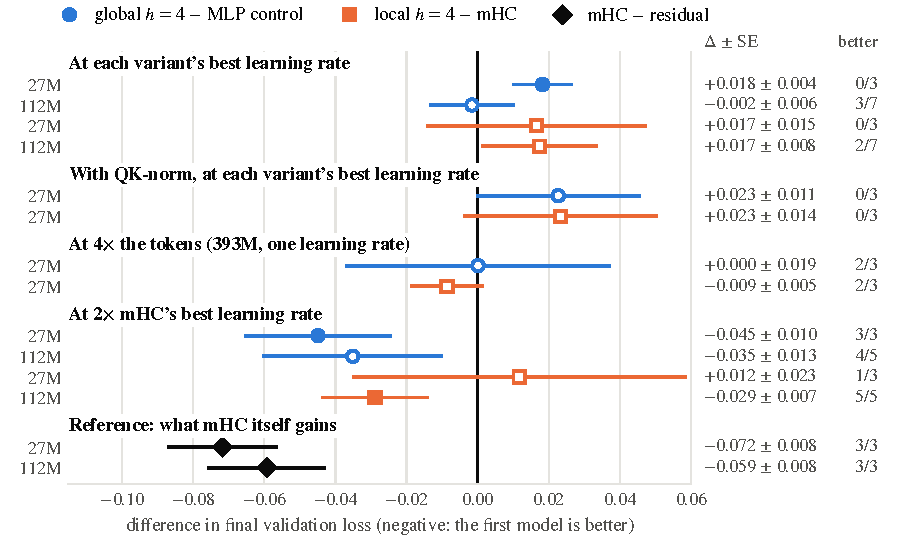
\includegraphics[width=\linewidth]{summary}
  \caption{Summary of the main comparisons. Each row is a difference in final validation loss with the standard error of
    \cref{sec:stats}, shown as the mean $\pm$ 2 SE over seeds, with filled markers for established effects. The columns on the right
    give the mean $\pm$ SE and the number of seeds on which the first model is better. All groups except the second are without
    QK-norm, and the 112M rows other than mHC $-$ residual pool two TPU generations (\cref{app:chips}). With every model at its own
    best learning rate the heads gain nothing at equal parameters. They lead only above the optimal learning rate, and only without
    QK-norm (\cref{sec:tolerance} and~\cref{sec:qknorm}).}
  \label{fig:main}
\end{figure}

Multi-head attention showed that several smaller attention heads, each with its own projections, can work better than a single
head of full width at a similar cost \citep{vaswani2017attention}. The same split applied to mHC gives multi-head mHC
(\cref{sec:design}). The $D$ channels are cut into $h$ groups, and each group gets its own read, write and doubly stochastic mix.
The design keeps the guarantees of mHC, group by group (\cref{sec:guarantees}), and seen through depth it gives each group of
channels its own pattern of connections to earlier layers (\cref{sec:depth}).

This paper asks whether multi-head mHC gives a better model for the same parameters and compute. We ran a controlled study at 27M
and 112M parameters, 629 training runs on TPU v5e and v6e. Runs are paired by seed, every model that adds parameters is
compared with a control that spends the same parameters on a wider feed-forward layer, and every main variant has a learning-rate
grid at both widths. At 27M we also repeat the grid with QK-norm, ablate the per-head blocks and train with four times the tokens.
Decision rules were written down before the results they decide. They are public, with the code and the results of every run
(\cref{app:implementation}).

The answer is no (\cref{fig:main}). With every model at its own best learning rate, heads at the parameter count of mHC are no
better than mHC, and heads that add parameters are no better than mHC with a feed-forward layer widened to the same count. This
holds at both widths, at 27M with QK-norm, and at one learning rate with four times the tokens. None of the three per-head blocks,
kept alone, uses its parameters better than the feed-forward layer (\cref{sec:parts}). Compared in the more common way, at one
shared learning rate and without a parameter-matched control, the same heads beat mHC on 9 of 10 seeds by about 40\% of mHC's gain
over the residual connection. It takes both controls to see that this gain comes from the extra parameters and the choice of
learning rate (\cref{sec:fixed-lr} and~\cref{sec:lesson}).

The heads change how training fails when the learning rate is too high. Without QK-norm they lose less than mHC above the optimal
learning rate, and robustness of this kind, measured in smaller models, has been used as a proxy for the instabilities of large
runs \citep{wortsman2023proxies, qiu2026qwen38next}. We tested whether it amounts to a stability benefit and find no evidence that
it does (\cref{sec:tolerance}, \cref{sec:qknorm} and~\cref{sec:scale}). Above the optimum every variant fails through
attention-logit growth, and the heads do not prevent it. QK-norm, which current open models use, removes the failure, and with
QK-norm the heads are more sensitive to the learning rate than mHC. In the stability test only one run, which fails, has loss
spikes. The one difference that survives QK-norm is that the heads keep the gradient norm below the clipping threshold where that
of mHC occasionally crosses it. This does not show in the loss, and whether it would matter in a large model is untested.

\section{Related Work}
\label{sec:related}

Most follow-up work on HC and mHC re-parameterizes the single $n \times n$ mix over the copies \citep{yang2026mhclite,
zhou2026kromhc, dandachi2026gomhc, lyubinin2026tbpmhc, liu2026shc, guo2026ohc} or the dense maps that predict the coefficients
\citep{gu2026temper}. Other work raises the number of copies while updating only a few of them per sublayer \citep{zhang2026xhc}
or carries a static form of mHC to state space models \citep{mutlu2026mhcssm}. Some designs use channel groups as the streams
themselves \citep{zhu2025fracconnections} or widen the stream and split it into such groups \citep{seed2025vwn}, with one shared
mix in both. None of them gives each group of channels its own copies and its own mix. In a trained mHC model a typical site uses
only about two of its four streams \citep{zhao2026howdoesmhc}, and when the copies start identical they can collapse onto a
dominant one \citep{alimaskina2026streamcollapse}.

The value of the mix itself has been questioned. Several recent designs drop it \citep{qiu2026qwen38next, ge2026chimera,
liang2026sihc}, and a concurrent submission finds that learned read and write gates with the mix fixed to the identity match mHC
\citep{anon2026simplehc}. Another shows that constraining one marginal of the mixes already bounds the norm of their product at
any depth \citep{anon2026oshc}.

\Cref{tab:related} lists the designs closest to ours by where their coefficients are shared. The gated residual of Qwen3.8-Next
\citep{qiu2026qwen38next} reads a four-branch stream through an elementwise gate and writes with one scalar per branch, without a
mix. Its read has the granularity of ours at $h = D$. The ablations in that work find the granularity of the read more useful than
that of the write, and the mix of little value once the read and write are expressive. SiHC \citep{liang2026sihc} uses static
per-channel read and write maps, with the mix fixed to the identity, in pixel diffusion transformers whose streams hold different
subpatches. uHC \citep{anon2026uhc}, a concurrent submission, argues, as our design assumes, that readout patterns shared across
feature dimensions are a bottleneck. It computes the read of each group of channels from that group's own slice of the copies,
which is our per-head read with a local predictor, and adds a low-rank write-back with extra parameters while keeping the mix of
mHC. Its validation loss is lower than that of mHC by 0.006 and 0.008 at 46M and 128M parameters and by 0.128 at 363M, where its
mHC baseline is 0.093 worse than the residual connection. All methods share one learning rate per scale, and no seed count is
reported. \Cref{sec:parts} tests the per-head read alone, with a global predictor, against a parameter-matched control. The
per-group mix is the one part of our design that none of these has.

\begin{table}[ht]
  \centering
  \caption{Where the connection coefficients are shared in the designs closest to multi-head mHC. ``Shared'' means one
    coefficient per copy for all channels. The mix is one $n \times n$ matrix over the copies, doubly stochastic in mHC and in our
    design.}
  \label{tab:related}
  \small
  \begin{tabular}{llll}
    \toprule
    design & read & write & mix \\
    \midrule
    HC \citep{zhu2024hyperconnections}, mHC \citep{xie2026mhc} & shared & shared & shared \\
    Qwen3.8-Next gated residual \citep{qiu2026qwen38next} & per channel & shared & none \\
    SiHC \citep{liang2026sihc} & per channel, static & per channel, static & identity \\
    uHC \citep{anon2026uhc}, concurrent & per group & shared plus low-rank & shared \\
    \midrule
    multi-head mHC (ours) & per group & per group & per group \\
    \bottomrule
  \end{tabular}
\end{table}

The same split has been applied to other connections. Multi-Head Attention Residuals \citep{luo2026mhar} split the depth-attention
query of Attention Residuals \citep{kimi2026attnres} into channel groups with independent routers. Their loss is U-shaped in the
number of heads with its minimum at 4--8, and the gain survives per-method learning-rate tuning at 100M--1B parameters. An
anonymous submission with the same title \citep{anon2026mharICLR} adds temperature-matched controls, which attribute most of the
gain of the split over a single query to the flatter softmax of each smaller head and only a small part to routing each subspace
separately. The report that introduced Attention Residuals tested the same split with 16 heads and found a slightly higher loss
(1.752 against 1.746), concluding that the best mixture over depth is largely uniform across channels \citep{kimi2026attnres}. In
Depth-Attention \citep{zeng2026depthattention}, per-head softmax mixing over depth improves only slightly on a fixed uniform
average of the same layers, and Kimi K3 \citep{kimi2026k3} ships single-head Attention Residuals.

Small-scale comparisons of residual variants depend on how they are controlled. A per-channel residual gate compared against
parameter-matched baselines was within noise up to 320M parameters, significant at 590M and only a trend at 1B
\citep{kramer2026reviewresiduals}. With the learning rate tuned per architecture at 400M parameters, the best learning rate of mHC
equals that of the pre-norm residual \citep{wang2026depthbench}. More broadly, most of the transformer modifications that
\citet{narang2021modifications} reimplemented in one shared code base did not meaningfully improve performance, and
well-regularized standard LSTMs outperformed more recent recurrent architectures in language modeling once all of them were tuned
by the same large-scale hyperparameter search \citep{melis2018evaluation}. We also tune the learning rate of each variant and find
that this choice decides the result (\cref{sec:best-lr}).

Raising the learning rate reproduces in small models two instabilities first seen in large ones \citep{wortsman2023proxies}. In
the first, attention logits grow until attention collapses onto one key. This appeared at about 8B parameters while vision
transformers were scaled to 22B \citep{dehghani2023vit22b} and is known as attention entropy collapse
\citep{zhai2023entropycollapse}. In the second, the output logits drift. A normalization of the queries and keys, QK-norm, removes
the first and a z-loss the second. QK-norm was introduced for translation \citep{henry2020qknorm}, was applied in a LayerNorm form
to attention-logit growth by \citet{dehghani2023vit22b} and is now standard in open models \citep{olmo2024olmo2, gemma2025gemma3,
yang2025qwen3}. Qwen3.8-Next stress-tests its new architecture and optimizer against the structure they replace at two to four
times the optimal learning rate and counts loss spikes and clipped steps \citep{qiu2026qwen38next}. We use the same measures to
ask whether the tolerance of the heads to a too-high learning rate is a stability benefit (\cref{sec:tolerance}, \cref{sec:qknorm}
and~\cref{sec:scale}).

\section{Method}
\label{sec:method}

\subsection{Background on mHC}
\label{sec:mhc}

Per token, the residual stream is $X \in \mathbb{R}^{n \times D}$, made of $n$ copies of width $D$ ($n = 4$ unless stated
otherwise). A sublayer $F$, either attention or feed-forward, is wrapped as
\begin{equation}
  u = \Hpre X, \qquad y = F(u), \qquad X' = \Hres{}^{\top} X + \Hpost{}^{\top} y,
  \label{eq:mhc}
\end{equation}
with a read $\Hpre \in \mathbb{R}^{1 \times n}$, a write $\Hpost \in \mathbb{R}^{1 \times n}$ and a mix $\Hres \in \mathbb{R}^{n
\times n}$. In mHC the three are predicted per token from the RMS-normalized, flattened stream by three linear maps, each scaled
by a learned $\alpha$ and added to a static bias. Then $\Hpre = \sigma(\cdot)$, $\Hpost = 2\sigma(\cdot)$ and $\Hres =
\mathrm{Sinkhorn}(\exp(\cdot))$, which is doubly stochastic up to the accuracy of the Sinkhorn iteration \citep{xie2026mhc}. A
doubly stochastic matrix has spectral norm at most 1 and preserves the sum over the copies, and a product of such matrices is
again doubly stochastic. The mix composed over any number of layers therefore stays bounded.

\subsection{Multi-head mHC}
\label{sec:design}

We split the $D$ channels into $h$ contiguous groups of $D/h$ channels and give each group its own read, write and doubly stochastic
mix. \Cref{eq:mhc} is applied to the $n \times D/h$ block of the stream that belongs to group $g$, $X_{(g)}$, and to the
matching block of the sublayer output, $y_{(g)}$,
\begin{equation}
  u_{(g)} = \Hpre_{(g)} X_{(g)}, \qquad y = F\bigl([u_{(1)}, \ldots, u_{(h)}]\bigr), \qquad
  X'_{(g)} = \Hres_{(g)}{}^{\top} X_{(g)} + \Hpost_{(g)}{}^{\top} y_{(g)}.
  \label{eq:multihead}
\end{equation}
The sublayer is unchanged and reads the concatenation of the reads of all groups. With $h = 1$ the model is mHC.
\Cref{fig:method} shows one sublayer of each.

\begin{figure}[ht]
  \centering
  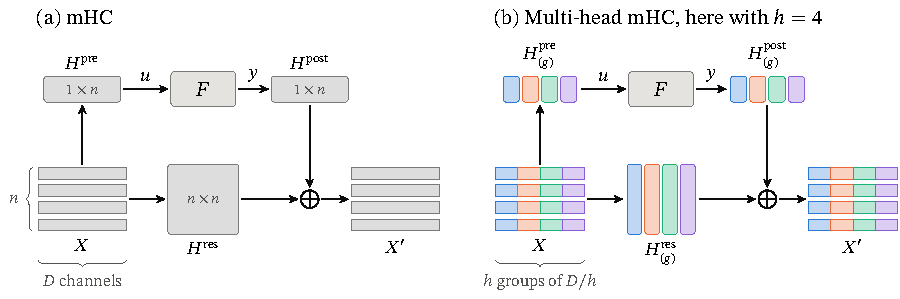
\includegraphics[width=\linewidth]{method}
  \caption{One sublayer of mHC (a) and of multi-head mHC (b). mHC reads the $n$ copies into the sublayer input $u$, mixes them and
    writes the output $y$ back, with one coefficient per copy for all $D$ channels. Multi-head mHC gives each of the $h$ channel
    groups (shown in different colors) its own read, mix and write. The sublayer $F$ is the same in both.}
  \label{fig:method}
\end{figure}

\subsection{Guarantees}
\label{sec:guarantees}

On $\mathrm{vec}(X)$, with the channels of each group kept together, the mixing operator of \cref{eq:multihead} is block diagonal,
\begin{equation}
  \operatorname{diag}\bigl(\Hres_{(1)}{}^{\top} \otimes I_{D/h},\; \dots,\; \Hres_{(h)}{}^{\top} \otimes I_{D/h}\bigr).
  \label{eq:blockdiag}
\end{equation}
Its spectral norm is the largest of those of its blocks, which is at most 1. Each block preserves the sum over copies of its own
channels, and a product of such operators is again block diagonal with doubly stochastic blocks. All three properties of mHC
therefore hold, group by group.

\subsection{A depth view}
\label{sec:depth}

Unrolling \cref{eq:mhc} shows that sublayer $l$ reads a weighted sum of the embedding and all earlier outputs,
\begin{equation}
  u_l = \sum_{s < l} c_{ls}\, y_s, \qquad
  c_{ls} = \Hpre_l\, \Hres_{l-1}{}^{\top} \cdots \Hres_{s+1}{}^{\top}\, \Hpost_s{}^{\top},
  \label{eq:depth}
\end{equation}
where $y_0$ is the embedding. The plain residual has $c \equiv 1$. DenseFormer learns $c$ directly
\citep{pagliardini2024denseformer} and MUDDFormer predicts it from the hidden state \citep{xiao2025muddformer}. In mHC the copies
act as a state of size $n$ carried through depth, which is written by $\Hpost$, moved by $\Hres$ and read by $\Hpre$. The matrix
$c$ is therefore $n$-semiseparable, meaning that every block below its diagonal has rank at most $n$. mHC gives all $D$ channels
one such pattern, and $h$ heads give each channel group its own. Raising $n$ instead raises the rank of the single pattern, at the
cost of a wider stream.

\subsection{Predictors and parameter cost}
\label{sec:predictors}

How the coefficients of each group are produced is a separate choice. A \emph{local} predictor computes the coefficients of group
$g$ from its own $n \times D/h$ slice of the stream and has the parameters of mHC, cut into $h$ blocks. A \emph{global} predictor
computes the coefficients of every group from the whole stream and has $h$ times the parameters of the mHC predictor. A
\emph{static} predictor uses the biases only. \Cref{tab:params} gives the parameter counts. At $D = 384$, global $h = 4$ adds 1.8M
parameters to mHC (6.5\%) and $h = 16$ adds 9M (33\%), so every model with global heads needs a control with the same parameter
count (\cref{sec:controls}).

\begin{table}[ht]
  \centering
  \caption{Parameter counts of the main models at the two widths.}
  \label{tab:params}
  \small
  \begin{tabular}{lrr}
    \toprule
    model & $D = 384$ & $D = 768$ \\
    \midrule
    residual connection & 26.75M & 110.12M \\
    mHC & 27.34M & 111.90M \\
    local $h = 4$ & 27.34M & 111.90M \\
    global $h = 4$ & 29.13M & 117.25M \\
    MLP control for global $h = 4$ (mHC, SwiGLU width 1216 / 2240) & 29.11M & 117.21M \\
    global $h = 16$ & 36.29M & -- \\
    MLP control for global $h = 16$ (mHC, SwiGLU width 1992) & 36.26M & -- \\
    \bottomrule
  \end{tabular}
\end{table}

\subsection{Ablations and other variants}
\label{sec:variants}

Any subset of the three blocks can be made per head while the others are predicted once and shared by all groups. With no block
per head the model is exactly mHC, and with only the read per head and a local predictor it is the group-wise readout of uHC
\citep{anon2026uhc}. We tested two side variants. The first is a joint $(nh) \times (nh)$ doubly stochastic mix over (copy, group)
pieces, which lets groups exchange channels. The second is mHC with $n = 8$ copies. Mixtures of several Sinkhorn matrices add
nothing over a single one, since the doubly stochastic matrices form a convex set.

\section{Experimental Setup}
\label{sec:setup}

\subsection{Models, data and training}
\label{sec:training}

The models are pre-norm GPTs with rotary attention, SwiGLU feed-forward layers and an untied output layer (\cref{tab:setup}). They
are trained on FineWeb-Edu with a 16,384-token BPE vocabulary, using random 1024-token windows from a 200M-token pool, and validated
on a fixed set of 819k tokens. Training uses AdamW with $\beta = (0.9, 0.95)$ and weight decay 0.1 on matrices, 200 warmup steps,
cosine decay to 10\% of the peak learning rate and gradient clipping at 1.0. Each run takes 6000 steps of $16 \times 1024$ tokens,
or 98M tokens. The connection runs in float32 and the rest of the model in bf16. mHC follows the published recipe, with
$n = 4$, 20 Sinkhorn iterations, $\alpha$ initialized to 0.01 and an initialization close to the pre-norm residual.

For the stability test of \cref{sec:tolerance} and~\cref{sec:qknorm}, the five main variants at 27M are also trained with QK-norm,
an RMSNorm on the queries and keys of each attention head before the rotary embedding. Gemma~3 and Qwen3 also use QK-norm
\citep{gemma2025gemma3, yang2025qwen3}, and OLMo~2 applies it to the whole query and key projections rather than to each head
\citep{olmo2024olmo2}. These runs use nine learning rates from \lr{1.5} to \lr{24} spaced by a factor of about $\sqrt{2}$, and the
grid without QK-norm is extended to the same top. They log the loss and the gradient norm before clipping at every step. Every 250
steps they log the largest attention logit and the mean attention entropy of every layer on four fixed validation sequences.

\begin{table}[ht]
  \centering
  \caption{The two model sizes and their training.}
  \label{tab:setup}
  \small
  \begin{tabular}{lll}
    \toprule
    & 27M & 112M \\
    \midrule
    width $D$ / layers / attention heads & 384 / 8 / 6 & 768 / 12 / 12 \\
    SwiGLU width & 1024 & 2048 \\
    tokens & 98M, and 393M for one test & 98M \\
    learning rates ($\times 10^{-3}$) & 1.5, 2.1, 3, 4.2, 6 & 0.53, 0.75, 1.06, 1.5, 2.1 \\
    stability test ($\times 10^{-3}$) & 1.5 to 24, QK-norm on and off & -- \\
    seeds per learning rate & 3 (v6e), 2--10 (v5e) & 3 (v6e, 5 at the best), 2 (v5e) \\
    TPU & v6e and v5e & v6e and v5e \\
    \bottomrule
  \end{tabular}
\end{table}

\subsection{Baselines, controls and learning rates}
\label{sec:controls}

Every comparison includes mHC and the plain residual connection. Global heads add parameters, so each is compared with mHC widened
in the feed-forward layer to the same parameter count, which we call the \emph{MLP control} (\cref{tab:params}). Local heads have
the parameter count of mHC and are compared with mHC directly. For other variants we use the \emph{MLP line}, which is linear in the
parameter count and passes through mHC and its widened versions. It gives the loss that the same parameters buy in the feed-forward
layer.
\label{sec:lrs}

The first experiments used a single peak learning rate, \lr{3}, which was the best for mHC in a pilot. We then mapped the learning
rate of mHC, global and local $h = 4$, the MLP control and the residual, so that each can be compared at its own best. The best
learning rate is the one with the lowest mean final loss over seeds 0--2, a rule fixed in advance.

\subsection{Statistics and hardware}
\label{sec:stats}
\label{sec:hardware}

For a given seed, every variant starts from the same weights outside the connection and sees the same batches, so differences at
the same learning rate are paired by seed. We report the mean difference in final validation loss with its standard error and
the number of seeds on which the first model is better. We call an effect \emph{established} when $|\text{mean}| > 2$\,SE and
all seeds agree in sign, a rule fixed before the main runs. Comparisons between variants at different learning rates, and all
comparisons at the best learning rates at $D = 768$, use the two-sample standard error. Where both chips ran the same
comparison, we pool the two by inverse variance as independent estimates.

Every run uses one TPU chip, either v5e or v6e. The two chips are not interchangeable, since the same run on v6e behaves like a
new seed of the v5e run. Each experiment therefore stays on one chip type with its own baselines, and we never compare numbers
from different chips directly (\cref{app:chips,app:implementation}).

\section{Results}
\label{sec:results}

\subsection{Comparison at equal parameters}
\label{sec:matched}
\label{sec:best-lr}

We compare local heads with mHC and global heads with the MLP control (\cref{sec:controls}), with every variant at its own best
learning rate, which is the fair setting, and at one learning rate shared by all, which is the usual setting for connection
variants.

The learning-rate grids put the optimum of mHC, global $h = 4$, the MLP control and the residual at \lr{2.1} at 27M on TPU v6e.
Local $h = 4$ is best at \lr{3}, ahead of its value at \lr{2.1} by 0.003 (\cref{fig:lr}, left). At 112M the optimum is \lr{0.75}
for mHC, local $h = 4$ and the control. Global $h = 4$ and the residual are best at \lr{1.06}, ahead of their values at \lr{0.75}
by 0.0008 and 0.0016, and the v5e grid, which has the residual only at \lr{1.5}, puts every optimum in the same place
(\cref{fig:lr}, right, and \cref{app:grids}). The heads move neither the optimum nor the range of learning rates within 0.02 of
it. At 27M this range covers two grid points for mHC and both head variants and three for the control and the residual. At 112M it
covers three points for global $h = 4$, two for mHC, the control and the residual and one for local $h = 4$.

\begin{figure}[ht]
  \centering
  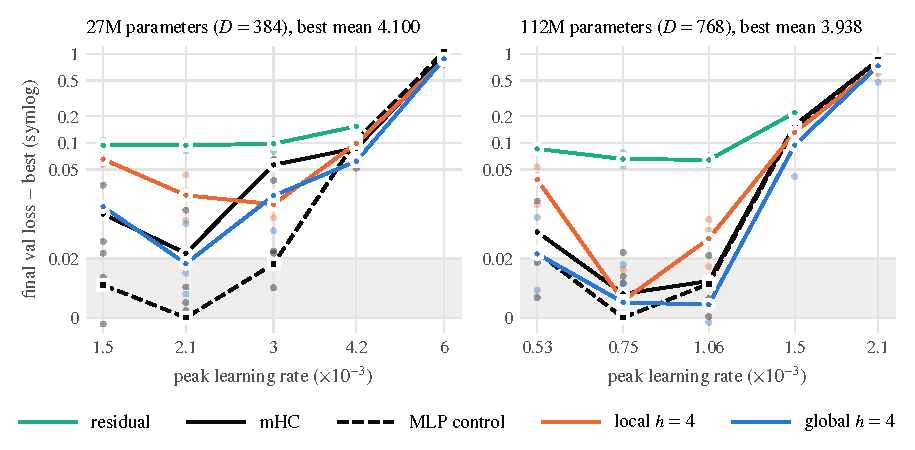
\includegraphics[width=\linewidth]{lr}
  \caption{Final validation loss above the best mean at each width, against the peak learning rate (TPU v6e, 98M tokens). Lines
    show the mean over seeds 0--2 and dots show single seeds. The axis is symlog and linear below 0.05, and the shaded band marks
    losses within 0.02 of the best variant. The heads move neither the optimum nor the range of good learning rates. Just above the
    optimum, at \lr{4.2} and \lr{1.5}, global $h = 4$ lies below mHC and the control.}
  \label{fig:lr}
\end{figure}

\Cref{tab:best-lr} compares the variants at these optima. At 27M the MLP control is ahead of global $h = 4$ on every seed, by
$0.018 \pm 0.004$, so at their best the heads are worth less than their parameters. At 112M the two are level on both chips, and
pooled over 7 seeds the difference is $-0.002 \pm 0.006$. Local heads are no better than mHC at either width ($+0.017 \pm 0.015$ and
$+0.017 \pm 0.008$). The gain of mHC over the residual holds at both widths ($-0.072 \pm 0.008$ and $-0.059 \pm 0.008$) and at every
learning rate of both grids.

\begin{table}[ht]
  \centering
  \caption{Each variant at its own best learning rate. Global and local denote $h = 4$, and control denotes the MLP control. At 27M
    (TPU v6e, seeds 0--2) differences are paired where the two learning rates coincide. At 112M they use two-sample standard errors,
    with 5 seeds on v6e (3 for the residual) and 2 on v5e, pooled by inverse variance. $\est$ marks established effects.}
  \label{tab:best-lr}
  \small
  \setlength{\tabcolsep}{4pt}
  \begin{tabular}{lcccc}
    \toprule
    & 27M & \multicolumn{3}{c}{112M} \\
    \cmidrule(lr){2-2} \cmidrule(lr){3-5}
    comparison & v6e & v6e & v5e & pooled \\
    \midrule
    global $-$ control & $+0.018 \pm 0.004\est$ (0/3) & $+0.006 \pm 0.007$ (1/5) & $-0.016 \pm 0.011$ (2/2) & $-0.002 \pm 0.006$ \\
    local $-$ mHC & $+0.017 \pm 0.015$ (0/3) & $+0.013 \pm 0.011$ (2/5) & $+0.023 \pm 0.012$ (0/2) & $+0.017 \pm 0.008$ \\
    global $-$ mHC & $-0.004 \pm 0.013$ (1/3) & $-0.005 \pm 0.008$ (3/5) & $-0.007 \pm 0.010$ (1/2) & $-0.006 \pm 0.006$ \\
    control $-$ mHC & $-0.022 \pm 0.011$ (3/3) & $-0.010 \pm 0.010$ (4/5) & $+0.010 \pm 0.013$ (0/2) & $-0.004 \pm 0.008$ \\
    mHC $-$ residual & $-0.072 \pm 0.008\est$ (3/3) & $-0.059 \pm 0.008\est$ (3/3) & -- & -- \\
    \bottomrule
  \end{tabular}
\end{table}

The result is the same at a shared learning rate. At \lr{3}, the pilot rate of mHC, on TPU v5e (\cref{tab:fixed-lr}), local heads
land within 0.003 of mHC at $h = 2$ (10 seeds) and $h = 4$ (6 seeds), and static heads gain nothing over static mHC ($-0.003 \pm
0.006$). Global $h = 4$ is level with its control over 10 seeds ($+0.005 \pm 0.007$), and with these seeds a difference of about
0.015 would have been detected. Global $h = 16$ trails its control on every seed ($+0.046 \pm 0.004$), so the same parameters gain
3.4 times as much in the feed-forward layer.

QK-norm does not change the comparison (\cref{sec:qknorm}). On a nine-point grid at 27M, with every variant at its own best learning
rate, local $h = 4$ trails mHC by $0.023 \pm 0.014$ and global $h = 4$ trails the control by $0.023 \pm 0.011$, better on 0 of 3
seeds in each case. A planned repeat at 112M could not be run (\cref{sec:limitations}).

\subsection{Longer training}
\label{sec:long}

All results so far use 98M tokens, or 3.6 tokens per parameter at $D = 384$. To test the effect of training length, we trained mHC,
global and local $h = 4$, the MLP control and the residual on 393M tokens (14 per parameter) at \lr{3}, with seeds 0--2 on TPU v5e.
These runs keep the same warmup and stretch the cosine decay over the longer run, and the comparisons were fixed beforehand. Each
token of the pool is seen about twice, and every variant sees the same batches. The 98M-token runs of the same variants, chip,
learning rate and seeds provide the shorter length (\cref{tab:long}).

\begin{table}[ht]
  \centering
  \caption{Comparisons at four times the tokens. $D = 384$ at 98M and 393M tokens (TPU v5e, \lr{3}, seeds 0--2), paired by seed.
    The last column gives the per-seed change from 98M to 393M tokens, which is negative when the first model gains relative to the
    second with longer training. $\est$ marks established effects.}
  \label{tab:long}
  \small
  \setlength{\tabcolsep}{4pt}
  \begin{tabular}{lccc}
    \toprule
    comparison & 98M tokens & 393M tokens & change \\
    \midrule
    global $h = 4$ $-$ MLP control & $+0.017 \pm 0.024$ (1/3) & $+0.000 \pm 0.019$ (2/3) & $-0.017 \pm 0.011$ (2/3) \\
    local $h = 4$ $-$ mHC & $-0.006 \pm 0.008$ (2/3) & $-0.009 \pm 0.005$ (2/3) & $-0.003 \pm 0.005$ (2/3) \\
    global $h = 4$ $-$ mHC & $-0.024 \pm 0.005\est$ (3/3) & $-0.023 \pm 0.007\est$ (3/3) & $+0.001 \pm 0.011$ (1/3) \\
    MLP control $-$ mHC & $-0.041 \pm 0.024$ (2/3) & $-0.023 \pm 0.023$ (2/3) & $+0.018 \pm 0.001\est$ (0/3) \\
    mHC $-$ residual & $-0.041 \pm 0.007\est$ (3/3) & $-0.048 \pm 0.007\est$ (3/3) & $-0.007 \pm 0.003\est$ (3/3) \\
    \bottomrule
  \end{tabular}
\end{table}

Neither of the two comparisons of interest changes by an established amount. At 393M tokens global $h = 4$ and its control are tied
($+0.000 \pm 0.019$), and local heads are within noise of mHC ($-0.009 \pm 0.005$). The one established change is that the lead of
the control over mHC shrinks by 0.018 on every seed while the heads keep theirs, so the heads gain $0.017 \pm 0.011$ on the control
(2 of 3 seeds). On these seeds the lead of the control over the heads at 98M tokens (0.017) is larger than its ten-seed value
(0.005), so part of the shift is a return to the mean, and a single longer point with three seeds cannot show a trend. The gain of
mHC over the residual grows from 0.041 to 0.048. On v6e at 98M tokens the fixed learning rate lies above the optimum of every
variant except local $h = 4$, a regime in which the tolerance of the heads helps them, so if anything this setting favors the
heads.

\subsection{Variants that add parameters}
\label{sec:fixed-lr}

Compared with mHC, global heads look like an improvement. At \lr{3} on TPU v5e they beat mHC by about 0.02 at every $h$ from 2 to
16 (\cref{tab:fixed-lr}), roughly 40\% of the gain of mHC over the residual (0.045). At $h = 4$ the lead holds on 9 of 10 seeds.
The global predictor adds parameters, however, 1.8M at $h = 4$, and the MLP control gains as much with the same 1.8M in the
feed-forward layer ($-0.024 \pm 0.009$ against mHC). \Cref{fig:frontier} places every variant that adds parameters against the MLP
line. None lies below it by more than twice its standard error, and every way of spending parameters on the connection beyond $h =
4$, whether more heads, the joint mix or $n = 8$ copies, lies above it once it costs more than a few percent. In the TPU layout of
\cref{app:implementation} every head count runs at the speed of mHC (28.4k--29.3k against 28.7k tokens per second per chip), so
this is also a comparison at equal compute. With each model at its own best learning rate, even the raw lead over mHC disappears
($-0.004 \pm 0.013$ at 27M and $-0.006 \pm 0.006$ at 112M, \cref{tab:best-lr}). The gain at \lr{3} therefore comes from the extra
parameters, helped by a learning rate that lies above the optimum of mHC and global $h = 4$ in the v6e grid
(\cref{sec:tolerance}).

\begin{table}[ht]
  \centering
  \caption{All connection variants at one shared learning rate. Final validation loss relative to mHC at $D = 384$ and \lr{3} (TPU
    v5e, 98M tokens), paired by seed and given as mean $\pm$ SE. The last column counts the seeds on which the variant beats the
    reference. $\est$ marks established effects.}
  \label{tab:fixed-lr}
  \small
  \begin{tabular}{lrrlr}
    \toprule
    model & params & seeds & $\Delta$ loss & better \\
    \midrule
    residual connection & 26.75M & 4 & $+0.045 \pm 0.006\est$ & 0/4 \\
    static mHC & 26.75M & 3 & $+0.023 \pm 0.010\est$ & 0/3 \\
    static $h = 4$ & 26.75M & 3 & $+0.020 \pm 0.008\est$ & 0/3 \\
    static $h = 8$ & 26.75M & 3 & $+0.024 \pm 0.014$ & 0/3 \\
    joint mix, $h = 4$, static & 26.75M & 3 & $+0.013 \pm 0.008$ & 1/3 \\
    local $h = 2$ & 27.34M & 10 & $-0.003 \pm 0.009$ & 5/10 \\
    local $h = 4$ & 27.34M & 6 & $+0.003 \pm 0.008$ & 3/6 \\
    local $h = 8$ & 27.34M & 3 & $+0.010 \pm 0.017$ & 1/3 \\
    local $h = 16$ & 27.35M & 3 & $+0.003 \pm 0.010$ & 1/3 \\
    global $h = 2$ & 27.94M & 4 & $-0.020 \pm 0.009$ & 3/4 \\
    global $h = 4$ & 29.13M & 10 & $-0.019 \pm 0.006$ & 9/10 \\
    global $h = 8$ & 31.52M & 4 & $-0.021 \pm 0.011$ & 3/4 \\
    global $h = 16$ & 36.29M & 6 & $-0.019 \pm 0.005$ & 5/6 \\
    joint mix, $h = 4$, global & 33.85M & 3 & $-0.019 \pm 0.014$ & 2/3 \\
    mHC, $n = 8$ & 30.70M & 3 & $-0.006 \pm 0.011$ & 2/3 \\
    \midrule
    MLP control for global $h = 4$ & 29.11M & 10 & $-0.024 \pm 0.009$ & 8/10 \\
    MLP control for global $h = 16$ & 36.26M & 6 & $-0.065 \pm 0.007\est$ & 6/6 \\
    \midrule
    global $h = 4$ $-$ its control & & 10 & $+0.005 \pm 0.007$ & 2/10 \\
    global $h = 16$ $-$ its control & & 6 & $+0.046 \pm 0.004\est$ & 0/6 \\
    \bottomrule
  \end{tabular}
\end{table}

\begin{figure}[ht]
  \centering
  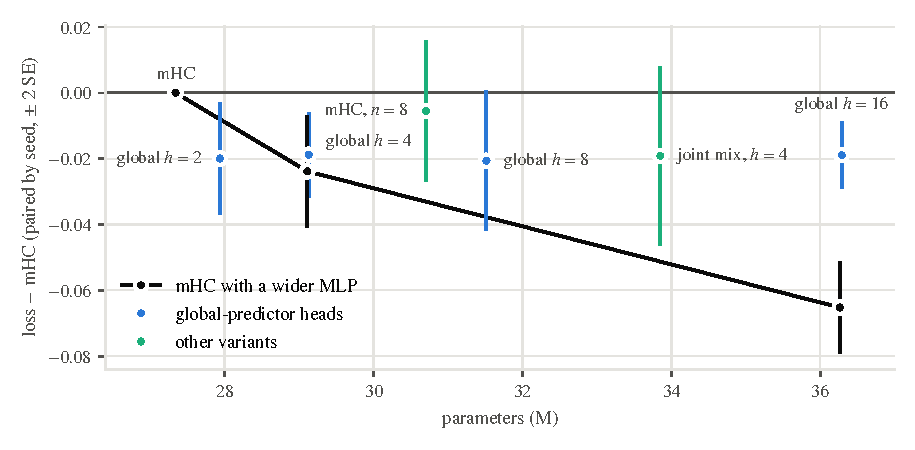
\includegraphics[width=\linewidth]{frontier}
  \caption{Loss relative to mHC of every variant that adds parameters, against its parameter count ($D = 384$, \lr{3}, TPU v5e,
    paired by seed, $\pm$ 2 SE). The black line is the MLP line, given by mHC with a wider feed-forward layer, and points above it
    use their parameters less well than the feed-forward layer does. Global heads gain about 0.02 over mHC at every $h$, whether
    they add 0.6M parameters or 9M, while the feed-forward layer turns the same 9M into a gain of 0.065. Variants at or below the
    parameter count of mHC are listed in \cref{tab:fixed-lr}.}
  \label{fig:frontier}
\end{figure}

\subsection{Behavior above the optimal learning rate}
\label{sec:tolerance}

The heads move neither the optimum nor the range of good learning rates (\cref{sec:best-lr}), but just beyond that range, where
every variant is at least 0.04 worse than its own best, they lose less. At 27M and \lr{4.2}, twice the optimum, global $h = 4$ is
$0.045 \pm 0.010$ ahead of its control (3 of 3 seeds, \cref{fig:main}), although it trails the control by 0.018--0.026 at every
lower learning rate of the grid (\cref{fig:lr}, left). At 112M and \lr{1.5}, again twice the optimum, global and local $h = 4$
lead mHC by 0.063 and 0.026 on every seed, and by 0.068 and 0.069 on v5e. The window is one grid point wide. At the next learning
rate, \lr{6} at 27M and \lr{2.1} at 112M, every variant run there ends 0.7--1.1 above its own best, and from \lr{8.5} at 27M runs
diverge or end more than 1 above the best. The heads therefore do not make a higher learning rate usable. They fail at the same
learning rate as the other models and lose less just before it. One of our early 112M results was an instance of this tolerance.
At \lr{1.5} on TPU v5e, half the 27M rate and untuned, global $h = 4$ led its control by $0.034 \pm 0.013$ (2 of 2 seeds), but
that rate is twice the optimum and costs every variant 0.09--0.18. Robustness to the learning rate in small models has been
proposed as a proxy for the instabilities of large runs \citep{wortsman2023proxies}. We therefore asked what fails, whether there
are loss spikes to count, and whether the tolerance survives QK-norm.

To see what fails, we replayed the 27M runs at \lr{2.1}, \lr{4.2} and \lr{6} with per-step logs and diagnostics
(\cref{sec:training}). All 42 replays reproduce the losses of the original runs bit for bit. Above the optimum, attention logits
grow until each head puts almost all of its weight on one key. This is the first of the two instabilities that
\citet{wortsman2023proxies} reproduce in small models \citep[see also][]{dehghani2023vit22b, zhai2023entropycollapse}. At step
1000 the largest attention logit is 47--77 at \lr{2.1}, 470--720 at \lr{4.2} and 1900--2700 at \lr{6} (\cref{fig:stability},
middle left), and the lowest mean attention entropy of any layer falls from 1.1--1.8 nats to 0.04--0.07 and then to 0.01. This
happens in every variant, and the heads do not slow it. At \lr{6}, global and local $h = 4$ reach 1930 and 2000, against 2070 for
mHC and 2470 for the residual. One layer behaves differently, which we noticed only after the fact. As in the residual, the first
attention layer of both head variants stays almost uniform at every learning rate (entropy 4.8--5.9 nats at \lr{6}, averaged over
seeds), while that of mHC and the control collapses with the rest (0.24).

We count loss spikes from the per-step logs in the ways used by OLMo~2 and Qwen3.8-Next \citep{olmo2024olmo2, qiu2026qwen38next}.
OLMo~2's spike score is the share of steps at least seven standard deviations away from the mean of the previous 1000. By this
measure only one run has loss spikes, seed 1 of mHC without QK-norm at \lr{8.5}, on 0.1\% of its steps, and that run ends 1.4
above the best loss of mHC. No other run with per-step logs that lasts beyond step 1000 has any, with or without QK-norm. The same
score for the gradient norm is below 0.5\% wherever training does not fail, and it is similar for all variants. The count used by
Qwen, steps more than 0.1 above a rolling median over 201 steps, does not separate the variants. At a batch of 16k tokens,
step-to-step noise crosses that threshold on about 8\% of steps at every learning rate, including the optimum.

We also asked whether the tolerance without QK-norm reflects slower connection dynamics. Scaling the learning rate of every
connection parameter by 0.25 changed nothing for mHC at any learning rate. Scaling it by 4 strengthened the tolerance instead of
removing it, and global $h = 4$ then ends 0.20 better than before at \lr{6} ($\pm 0.05$, 3 of 3 seeds). Because the decoupled weight
decay of AdamW scales with the learning rate, this setting also shrinks the weights of the predictor four times faster and pushes the
connection toward a static one. In a follow-up designed after seeing this result, and therefore exploratory, mHC with the same
setting gained nothing at \lr{6} ($+0.030 \pm 0.041$). At the optimum the setting changed neither model by more than the noise, and
global $h = 4$ stayed behind its control ($+0.007 \pm 0.005$, 0 of 3 seeds). The tolerance therefore belongs to the head split, and
a faster connection strengthens it only when the split is present.

\subsection{Effect of QK-norm}
\label{sec:qknorm}

With QK-norm no run diverges on the grid, up to \lr{24}, sixteen times its lowest point. The largest attention logit at step 1000,
averaged over seeds, stays between 15 and 26, and at \lr{24} every variant ends 0.18--0.21 above its own best
(\cref{fig:stability}, right). QK-norm also lowers the best loss of every variant, by 0.037--0.048. Above the optimum the heads
now lose more than mHC. We measure this with the learning-rate sensitivity of \citet{wortsman2023proxies}, the mean over the grid
of the final loss above the model's own best, with each loss capped at the loss at initialization, taken as $\ln 16384$. With
QK-norm, global and local $h = 4$ are more sensitive than mHC by $0.015 \pm 0.002$ and $0.006 \pm 0.003$, on each of the 3 seeds
(\cref{tab:stability}).

Without QK-norm the same measure is dominated by \lr{8.5}, where runs diverge on some seeds and not on others, and each divergence
adds about 0.47 to the sensitivity of a seed. Over the five learning rates up to \lr{6}, where no run diverges, the heads are less
sensitive than mHC without QK-norm (by $0.018 \pm 0.013$ and $0.028 \pm 0.010$) but not with it ($+0.004 \pm 0.001$ and
$+0.000 \pm 0.005$). By the rule we fixed before these runs, QK-norm removes the tolerance. Twelve runs without QK-norm, all at
\lr{8.5} or above, could not be run (\cref{sec:limitations}), but the verdict is the same whichever way they would have ended. With
QK-norm the heads also trail their parameter-matched baselines at all nine learning rates, global $h = 4$ the control by
0.011--0.052 and local $h = 4$ mHC by 0.006--0.066.

One difference between the heads and mHC survives QK-norm, and it is in the gradient norm. Papers on the HC family show
gradient-norm curves as evidence of stability \citep{xie2026mhc, yang2026mhclite, zhou2026kromhc, liu2026shc, lyubinin2026tbpmhc},
and there the heads differ from mHC (\cref{fig:stability}, bottom). Without QK-norm and at \lr{4.2}, the gradient norm before
clipping stays below 0.9 in the last 80\% of training for both head variants on every seed and below 1.6 for the residual, while
it reaches 6--16 for mHC and 6--20 for the control. At \lr{6}, where every variant fails, all of them cross the clipping threshold
on 29--84\% of those steps. With QK-norm the difference extends over the whole grid above the optimum of mHC. mHC crosses the
threshold on 0.03\% of the late steps at its best learning rate, \lr{1.5}, on 0.1\% at \lr{2.1}, which is still within 0.01 of its
best, and on 0.3--3\% from \lr{3} upwards. The control behaves in the same way. Global $h = 4$ crosses on almost none of the late
steps up to \lr{8.5} and on 0.4\% above it, local $h = 4$ on at most 0.15\% except at \lr{12} (0.9\%), and the residual on at most
0.1\%. Paired by seed, both head variants cross less often than mHC at every learning rate from \lr{2.1} to \lr{17} and on every
seed. These are small counts, since 0.1\% of the 4800 late steps is five steps.

The difference does not reach the loss. No run with QK-norm has a loss spike, clipping bounds every update, and with QK-norm mHC ends
below both head variants at every learning rate. Nor do the heads add a smoothness that the residual lacks. They remove a roughness
that mHC adds at 27M, although the authors of mHC report a gradient norm as steady as that of the residual at 27B
\citep{xie2026mhc}.

At 112M our data cannot settle the question. The 112M runs are without QK-norm and log every 25th step, which is too sparse to see
a rate like mHC's 0.1\% at 27M. From \lr{0.53} to \lr{1.5} no variant crosses on more than 1\% of the logged late steps, and the
residual, which almost never crosses at 27M, crosses most often at three of these four learning rates. At \lr{2.1}, 2.8 times the
optimum, where every variant has failed, the heads cross on 28--38\% and mHC on 85\%, as at 27M and \lr{6}. A repeat at 112M with
QK-norm and per-step logs could not be run (\cref{sec:limitations}).

\begin{table}[ht]
  \centering
  \caption{The stability test at 27M (TPU v6e, seeds 0--2). The column \emph{best} gives the best learning rate of each variant on
    the grid ($\times 10^{-3}$), \emph{logit} the largest attention logit over layers at \lr{6} and step 1000, averaged over seeds,
    and \emph{clipped} the share (\%) of steps in the last 80\% of training whose gradient norm before clipping exceeds 1.0, at
    \lr{4.2}. $\Delta S$ is the difference in the learning-rate sensitivity of \citet{wortsman2023proxies}, paired by seed and
    negative when the first variant is less sensitive. A diverged run counts as $\ln 16384$. Without QK-norm the full grid is
    complete only on the seeds shown, since twelve runs at \lr{8.5} and above could not be run. $\est$ marks established effects.}
  \label{tab:stability}
  \small
  \setlength{\tabcolsep}{4pt}
  \begin{tabular}{lcccccc}
    \toprule
    & \multicolumn{3}{c}{without QK-norm} & \multicolumn{3}{c}{with QK-norm} \\
    \cmidrule(lr){2-4} \cmidrule(lr){5-7}
    variant & best & logit & clipped & best & logit & clipped \\
    \midrule
    mHC & 2.1 & 2069 & 0.39 & 1.5 & 20.4 & 0.47 \\
    global $h = 4$ & 2.1 & 1926 & 0.00 & 3 & 18.7 & 0.00 \\
    local $h = 4$ & 3 & 2004 & 0.00 & 4.2 & 19.1 & 0.00 \\
    MLP control & 2.1 & 2710 & 0.68 & 2.1 & 20.4 & 0.49 \\
    residual & 2.1 & 2474 & 0.01 & 1.5 & 19.9 & 0.00 \\
    \midrule
    \multicolumn{7}{l}{$\Delta S$, all nine learning rates} \\
    \quad global $-$ mHC & \multicolumn{3}{c}{$-0.013$, $+0.472$ (seeds 0, 1)} & \multicolumn{3}{c}{$+0.015 \pm 0.002\est$ (0/3)} \\
    \quad local $-$ mHC & \multicolumn{3}{c}{$-0.067$, $-0.038$ (seeds 0, 1)} & \multicolumn{3}{c}{$+0.006 \pm 0.003\est$ (0/3)} \\
    \quad global $-$ control & \multicolumn{3}{c}{$-0.102$ (seed 0)} & \multicolumn{3}{c}{$+0.011 \pm 0.007$ (0/3)} \\
    \midrule
    \multicolumn{7}{l}{$\Delta S$, \lr{1.5} to \lr{6}} \\
    \quad global $-$ mHC & \multicolumn{3}{c}{$-0.018 \pm 0.013$ (2/3)} & \multicolumn{3}{c}{$+0.004 \pm 0.001\est$ (0/3)} \\
    \quad local $-$ mHC & \multicolumn{3}{c}{$-0.028 \pm 0.010\est$ (3/3)} & \multicolumn{3}{c}{$+0.000 \pm 0.005$ (2/3)} \\
    \quad global $-$ control & \multicolumn{3}{c}{$-0.048 \pm 0.012\est$ (3/3)} & \multicolumn{3}{c}{$+0.007 \pm 0.005$ (1/3)} \\
    \bottomrule
  \end{tabular}
\end{table}

\begin{figure}[ht]
  \centering
  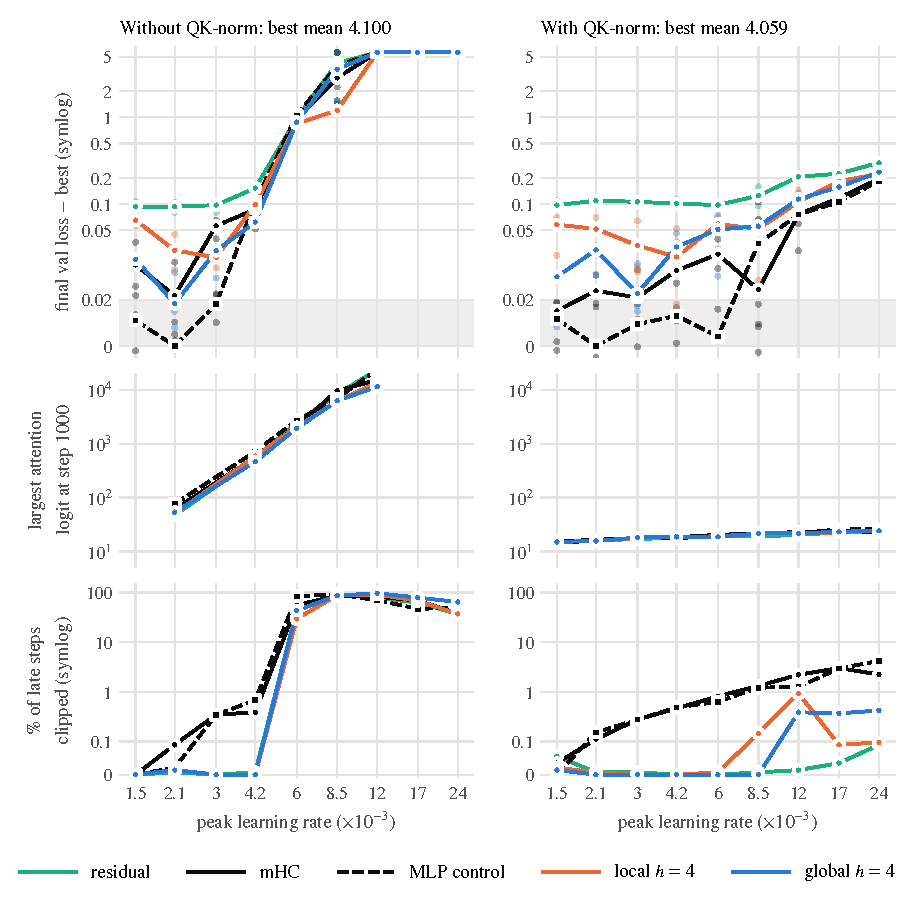
\includegraphics[width=\linewidth]{stability}
  \caption{The stability test at 27M, without QK-norm (left) and with it (right), at $D = 384$ on TPU v6e. The top row shows the
    final validation loss above the best mean of each panel against the peak learning rate. Lines show the mean over seeds 0--2, or
    over the seeds that ran where twelve runs without QK-norm at \lr{8.5} and above are missing, and dots show single seeds. The
    axis is symlog and linear below 0.05, and a diverged run counts as $\ln 16384$. The middle row shows the largest attention logit
    over layers at step 1000. The bottom row shows the share of steps in the last 80\% of training whose gradient norm before
    clipping exceeds 1.0, from every 25th step for the runs at \lr{1.5} and \lr{3} without QK-norm. The middle and bottom rows are
    averaged over seeds. QK-norm removes the failure and the tolerance of the heads, but not their smoother gradient norm.}
  \label{fig:stability}
\end{figure}

\subsection{Ablation of the per-head blocks}
\label{sec:parts}

Keeping only some of the three blocks per head separates their roles (\cref{fig:parts,tab:parts}). These runs were planned at
\lr{3}, the rate of the v5e experiments, before the grid showed that on v6e this rate lies above the optimum of mHC, global $h =
4$ and the control. We added the optimum, \lr{2.1}, after two of the three seeds at \lr{3} had finished, and ran it regardless of
what they showed.

\begin{table}[ht]
  \centering
  \caption{Global $h = 4$ with only some blocks per head ($D = 384$, TPU v6e, seeds 0--2). For each learning rate the table gives
    the paired difference to mHC and the excess over the MLP line at the parameter count of the variant, which is negative when the
    variant uses its parameters better than the feed-forward layer. $\est$ marks established effects.}
  \label{tab:parts}
  \small
  \setlength{\tabcolsep}{3.5pt}
  \begin{tabular}{lrccccc}
    \toprule
    & & \multicolumn{2}{c}{\lr{2.1} (optimum)} & \multicolumn{2}{c}{\lr{3}} & \lr{6} \\
    \cmidrule(lr){3-4} \cmidrule(lr){5-6} \cmidrule(lr){7-7}
    per head & params & $\Delta$ vs mHC & excess & $\Delta$ vs mHC & excess & $\Delta$ vs mHC \\
    \midrule
    read & 27.66M & $+0.002 \pm 0.015$ & $+0.006$ & $-0.025 \pm 0.011\est$ & $-0.019$ & $-0.012 \pm 0.022$ \\
    write & 27.64M & $-0.009 \pm 0.003\est$ & $-0.005$ & $-0.026 \pm 0.005\est$ & $-0.020$ & $-0.166 \pm 0.178$ \\
    read and write & 27.95M & $-0.002 \pm 0.001$ & $+0.006$ & $-0.029 \pm 0.005\est$ & $-0.016$ & $-0.179 \pm 0.060\est$ \\
    mix & 28.52M & $-0.001 \pm 0.009$ & $+0.014$ & $-0.015 \pm 0.004\est$ & $+0.011$ & $+0.066 \pm 0.112$ \\
    all three (global $h = 4$) & 29.13M & $-0.004 \pm 0.013$ & $+0.018$ & $-0.015 \pm 0.007\est$ & $+0.023$ & $-0.068 \pm 0.048$ \\
    \bottomrule
  \end{tabular}
\end{table}

At \lr{3} every split that keeps the mix shared beats mHC on every seed, by 0.025--0.029, and lies 0.016--0.020 below the MLP line,
so its few extra parameters appear better spent than in the feed-forward layer. The per-head mix alone costs 1.2M parameters, four
times as many as the read or the write, and buys less than those parameters would in the feed-forward layer. At \lr{6}, per-head
read and write with a shared mix keep 2.6 times the lead of the full split over mHC ($-0.18 \pm 0.06$, 3 of 3 seeds), and in the
last 80\% of training their gradient norm peaks lower than that of any other variant at that rate (5 on average over seeds,
against 16 for the full split and 51 for mHC). The per-head mix alone keeps none of the lead and peaks highest (93).

At the optimum the gains seen at \lr{3} are gone. No variant lies below the MLP line by more than twice its standard error, every
one trails the MLP control on every seed by 0.013--0.024, and the per-head read alone, which is the group-wise readout of uHC with
a global predictor, is $+0.002 \pm 0.015$ against mHC. The write alone comes closest. It beats mHC on every seed by $0.009 \pm
0.003$, but the MLP line gives 0.004 at its parameter count, and the remaining $-0.005$ falls short of $2\,\mathrm{SE} = 0.006$.
The gains at \lr{3} came from the same tolerance of a too-high learning rate that the full split shows, and they do not reflect a
better use of parameters.

\begin{figure}[ht]
  \centering
  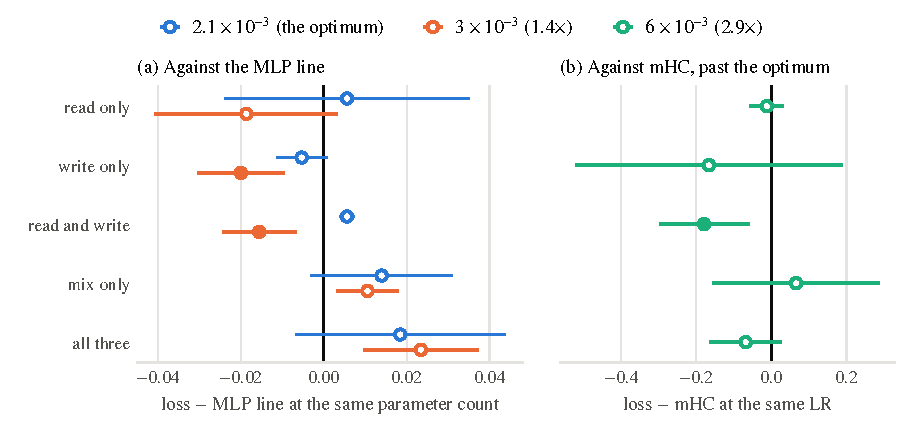
\includegraphics[width=\linewidth]{parts}
  \caption{Ablation of the per-head blocks (global predictor, $h = 4$, $D = 384$, TPU v6e, seeds 0--2, $\pm$ 2 SE). Filled
    markers show variants that beat the MLP line by more than 2 SE with every seed below it in (a), and established effects in (b).
    (a) At the optimum no block beats what its parameters buy in the feed-forward layer, while at 1.4 times the optimum the write
    alone and the read and write together do. (b) At 2.9 times the optimum only read and write per head with a shared mix keep a
    lead over mHC on every seed.}
  \label{fig:parts}
\end{figure}

A rule fixed before these results sent any read-only or read-and-write variant that beat the MLP line at \lr{3}, by more than twice
its standard error and on every seed, to $D = 768$. The read alone missed this bar (excess $-0.019$ against
$2\,\mathrm{SE} = 0.022$), and read and write together met it. At $D = 768$ and \lr{0.75}, read and write per head is
$-0.006 \pm 0.004$ against mHC (3 of 5 seeds), while the MLP line at its parameter count gives $-0.003$. This is an excess of
$-0.002$ against $2\,\mathrm{SE} = 0.008$, with 2 of 5 seeds below the line, and a difference of $+0.005 \pm 0.007$ against the full
control. The rule did not cover the write alone, which was therefore not run at $D = 768$.

\section{Discussion and Limitations}
\label{sec:discussion}

\subsection{Comparing connection variants}
\label{sec:lesson}

At the pilot learning rate of mHC, global heads looked like a clear improvement, 0.019 better than mHC on 9 of 10 seeds and about
40\% of the gain of mHC over the residual. Two controls removed this gain. The same parameters in a wider feed-forward layer gain
as much, and with every variant at its own best learning rate the lead disappears at both widths. What remained was an advantage
above the optimum, which describes how training fails and says little about the model one would train, and QK-norm removes it.
Connection variants are often compared at one shared learning rate and at unequal parameter counts. Our results suggest that both
controls are needed before a gain in this family is read as structural.

\subsection{Stability at larger scale}
\label{sec:scale}

A gentler failure above the optimum would be valuable if it predicted fewer instabilities in large models, where a failure costs a
whole run. Two lines of work make this argument plausible in general. \Citet{wortsman2023proxies} reproduce in small models, by
raising the learning rate, two instabilities first met in large models, and they measure the robustness of a model by its
learning-rate sensitivity, the expected excess loss over a learning-rate grid. Qwen3.8-Next accepts a new recipe only if a
28-layer mixture-of-experts model with 25B parameters (3B active) is at least as stable as the structure it replaces at two to
four times its optimal learning rate, counted in loss spikes and clip crossings, and the stability found there held in the
125B-parameter production model \citep{qiu2026qwen38next}. For four reasons, our results do not support the same argument for
multi-head mHC.

First, the failure we observe is one that QK-norm removes. Above the optimum our models fail through attention-logit growth, the
first of the two instabilities of \citet{wortsman2023proxies}, and the heads do not prevent it (\cref{sec:tolerance}). QK-norm
prevents it at every learning rate we tried, and with QK-norm the tolerance of the heads is gone (\cref{sec:qknorm}). Current open
models use QK-norm \citep{olmo2024olmo2, gemma2025gemma3, yang2025qwen3}, as Wortsman et al.\ do by default, so the property we
measured belongs to a recipe without this protection.

Second, the heads change how much the loss rises above the optimum but leave unchanged the learning rate at which models start
to fail. That learning rate is the quantity that Wortsman et al.\ show to depend on scale. It falls as models grow when attention logits
are not normalized, and they predict it by extrapolating the largest attention logit. The heads leave this learning rate
where mHC has it. Without QK-norm, mHC, both head variants and the residual first lose more than 0.1 at \lr{6}, and the control at
\lr{4.2}. With QK-norm all of them except the residual first do so at \lr{17}. Wortsman et al.\ also remark that in practice a lower
sensitivity matters little when the optimal learning rate does not change, since one can train at the optimum. With heads the
optimum stays where mHC has it, at both widths (\cref{sec:best-lr}).

Third, there are no loss spikes for the heads to reduce. Wortsman et al.\ study slow divergence and leave loss spikes out of
scope, tying them to the optimizer through the second-moment decay rate of Adam. Wherever training does not fail, none of the 27M
runs with per-step logs has a loss spike by the measure of OLMo~2 (\cref{sec:tolerance}). The spikes that matter at scale may also
have no small-scale counterpart. The Adam instability that dominated the training of a 546B model was absent at 7B and 30B
\citep{molybog2023adam}.

Fourth, the precedents differ from our case. In Qwen3.8-Next and in gated attention \citep{qiu2025gatedattention}, the more stable
design also had the lower loss in the comparisons reported, whereas multi-head mHC gives no gain at equal parameters. The stress
test of Qwen3.8-Next runs at 25B parameters, compares against a recipe already proven at scale and was confirmed in production,
whereas ours runs at 27M. The mechanism that the authors of Qwen3.8-Next credit is a bounded elementwise gate on what each layer
reads from the stream, and they drop the stream mix as a possible source of instability, which is the part that multi-head mHC
multiplies by $h$. At 7B and with QK-norm, OLMo~2 trained normally at two, three and four times its learning rate, and only ten
times was unstable \citep{olmo2024olmo2}. Sensitivity to the training hyperparameters measured in small models also shrinks with
scale \citep{lourie2026smallscale}.

The gradient norm is the one measure that favors the heads. They keep it under the clipping threshold where that of mHC crosses
it, with QK-norm as well (\cref{sec:qknorm}), and gradient-norm curves are part of how the HC family argues for stability. We
still cannot claim it as a benefit. What the heads remove at 27M is a roughness that mHC adds and the residual does not have, so
at most they restore the profile of the residual, which the authors of mHC report that mHC already has at 27B. The roughness costs
mHC nothing we can measure, since with QK-norm mHC has no loss spikes and a lower loss than the heads at every learning rate. Near
the optimum the difference does not show at 112M, the one larger model we have, although there we only have runs without QK-norm,
logged too sparsely to detect rates as low as those of mHC at 27M. To our knowledge, nobody has tested whether clip crossings in a
small model foretell loss spikes in a large one, and Qwen3.8-Next counts them in the large model itself.

What we can report is a gentler failure above the optimum and a smoother gradient norm. Neither is a stability benefit we can
claim for larger models. Testing either would require a model large enough to fail at its own tuned learning rate, or a stress test
at the scale of the one used for Qwen3.8-Next.

\subsection{Why the heads do not help}
\label{sec:elsewhere}
\label{sec:mix}

Head splits have helped in other connections. The same split applied to the depth read of Attention Residuals keeps a gain under
per-method tuning at 100M--1B parameters \citep{luo2026mhar}, although an anonymous submission with the same title attributes most
of the gain of the split over a single query to the flatter softmax of smaller heads and only a small part to routing each
subspace separately \citep{anon2026mharICLR}, and the authors of Attention Residuals found their own per-head version slightly
worse \citep{kimi2026attnres}. Per-channel reads helped in a mixture-of-experts model with 25B parameters (3B active) trained on
560B tokens \citep{qiu2026qwen38next} and in diffusion transformers whose streams hold different subpatches \citep{liang2026sihc}.
In mHC the copies start identical and trained models use only some of them at each site \citep{zhao2026howdoesmhc,
alimaskina2026streamcollapse}, so at our scale a per-group choice among the copies may have little to choose from. Consistent with
this, the per-group read alone is $+0.002 \pm 0.015$ against mHC at the optimum.

The per-group doubly stochastic mix is what separates our design from earlier and concurrent work, and it is also the block that
contributes least. It lies above the MLP line at both learning rates where we drew the line, it carries none of the tolerance
above the optimum, and it has the largest late gradient norm of the split variants there. This agrees with the recent designs that
drop the stream mix \citep{qiu2026qwen38next, ge2026chimera, liang2026sihc} and with the finding that read and write gates alone
match mHC \citep{anon2026simplehc}.

The tolerance needs the split, since a faster connection gives mHC none of it, and it sits in the per-group read and write. It is not
resistance to the failure itself, because attention logits grow as fast with heads as without them. A plausible explanation, which we
did not test, is that per-group coefficients let the connection turn down the channel groups whose updates grow too large, which a
single scalar per copy cannot do without silencing every channel at once. The one diagnostic in which the heads differ, a first
attention layer that stays almost uniform, is shared with the residual, which is not tolerant, so it explains at most part of the
effect. QK-norm makes the tolerance unnecessary.

\subsection{Limitations}
\label{sec:limitations}

Our models are small. They have 27M and 112M parameters and train on 98M tokens, 3.6 and 0.9 tokens per parameter, which is far
short of compute-optimal training for the larger one. The 393M-token runs, at one learning rate, with three seeds and with each
token seen about twice, are our only test of training length. The gain of Multi-Head Attention Residuals over the standard
residual was larger at 350M and 1B parameters than at 100M \citep{luo2026mhar}, and a per-channel residual gate first became
significant at 590M parameters \citep{kramer2026reviewresiduals}, so a gain at larger scale is not excluded.

The coverage of the study is also limited. All runs use one dataset, one tokenizer, $n = 4$ copies and contiguous channel groups.
Variants other than mHC, global and local $h = 4$, the control and the residual were run at one learning rate only. The control
widens the feed-forward layer, and another use of the same parameters, such as wider attention or more layers, could buy more or
less.

The comparisons rest on 3 to 10 seeds. Differences between global $h = 4$ and its control of about 0.015 at 27M (10 seeds at
\lr{3}) and 0.012 at 112M (7 seeds) would have been detected, but smaller structural effects are not excluded. With about twenty
variants and several learning rates per width, a few chance effects are expected, and one appeared and then vanished (local $h = 2$
at $-0.018$ on 4 seeds and $-0.003$ on 10). The comparisons that carry the conclusion are either far from the threshold or repeated
on a second chip.

The stability test runs at 27M only, with three seeds per learning rate, one batch size, AdamW with $\beta_2 = 0.95$, clipping at
1.0 and a 6000-step cosine schedule. It therefore cannot reproduce instabilities that appear only in long or large runs, or under a
constant learning rate as in Qwen's stress test. Twelve of its 240 runs, all without QK-norm at \lr{8.5} or above and all but
one on seed 2, could not be run for lack of spot TPU capacity. Every finished run in that range diverged except seven at \lr{8.5},
and the pre-registered verdict is the same for every possible outcome of the missing runs. A repeat at 112M with QK-norm and
per-step logs, planned to test the gradient-norm difference and the comparison at equal parameters, could not be run either, because
spot TPU capacity was too scarce and the VMs that did start were preempted before a run could finish. With QK-norm, mHC and the
residual are best at \lr{1.5}, the lowest point of the grid, so their true optimum may lie lower. That would only widen the lead of
mHC over local heads at the best learning rates. It would raise the sensitivity of mHC by as much as its best loss falls, which is
likely a small amount, since the loss of mHC changes by less than 0.01 from \lr{1.5} to \lr{3}.

Our results come from two TPU generations whose runs are not interchangeable (\cref{app:chips}). Each comparison stays on one of
them, and where both ran the same comparison we report both. Finally, we tested the group-wise read of the closest concurrent work
\citep{anon2026uhc} only with a global predictor and without its low-rank write-back.

\section{Conclusion}
\label{sec:conclusion}

Multi-head mHC gives each channel group its own read, write and doubly stochastic mix while keeping the guarantees of mHC. At
27M and 112M parameters, with every variant at its own best learning rate and against parameter-matched controls, it gives no
gain at equal parameters. With a global predictor it is worth at most what
its extra parameters are worth, and at the parameter count of mHC it is worth nothing. None of its blocks alone uses its parameters
better than the feed-forward layer, and at 27M neither QK-norm nor four times the tokens changes this.

Without QK-norm, multi-head mHC fails more gently at too-high learning rates, through the per-group read and write. This failure
is attention-logit growth, which the heads do not prevent. QK-norm removes it and makes the heads more sensitive to the learning
rate than mHC, and in the stability test only a run that failed had loss spikes, so we cannot offer the tolerance as a stability
benefit for larger models. The one difference that survives QK-norm is a smoother gradient norm, which does not reach the loss at
27M and which we could not test with QK-norm at 112M. Whether it matters at scale remains open, as does whether a gain at equal
parameters appears at billion-parameter scale, as other head splits suggest. At small scale the design adds nothing beyond its
parameters.

\renewcommand{\bibfont}{\small\raggedright}% the template's size; ragged, so long titles do not stretch the spaces
\renewcommand{\bibsection}{\section*{\refname}\phantomsection\addcontentsline{toc}{section}{\refname}\markboth{\refname}{}}
\bibliography{references}

\appendix

\section{Comparability Across Chips}
\label{app:chips}

TPU v5e, first on Kaggle and later on Google Cloud, ran the experiments of \cref{sec:fixed-lr}, the 393M-token runs, half of the
112M grid and a few 27M runs at other learning rates. On Google Cloud, a partial replay of a 27M run and a full replay of a 112M
Kaggle run were bit-identical at every logged step. All other TPU runs used spot TPU v6e. Before reading any v6e result, we
repeated on v6e the runs on which the $D = 384$ and $D = 768$ conclusions rested, with pass criteria fixed beforehand. Each run
had to fall within the seed-to-seed range of its variant on v5e, and each paired gap had to agree in sign and lie within the v5e
standard error.

\begin{table}[ht]
  \centering
  \caption{The same comparisons on the two chips. Paired gaps at $D = 384$ and \lr{3}, given as mean $\pm$ SE and the number of
    seeds on which the first model is better.}
  \label{tab:chips}
  \small
  \begin{tabular}{lccc}
    \toprule
    gap & v5e, all seeds & v5e, seeds 0--2 & v6e, seeds 0--2 \\
    \midrule
    global $h = 4$ $-$ mHC & $-0.019 \pm 0.006$ (9/10) & $-0.024 \pm 0.005$ (3/3) & $-0.015 \pm 0.007$ (3/3) \\
    global $h = 4$ $-$ MLP control & $+0.005 \pm 0.007$ (2/10) & $+0.017 \pm 0.024$ (1/3) & $+0.023 \pm 0.008$ (0/3) \\
    MLP control $-$ mHC & $-0.024 \pm 0.009$ (8/10) & $-0.041 \pm 0.024$ (2/3) & $-0.038 \pm 0.009$ (3/3) \\
    local $h = 4$ $-$ mHC & $+0.003 \pm 0.008$ (3/6) & $-0.006 \pm 0.008$ (2/3) & $-0.018 \pm 0.012$ (2/3) \\
    mHC $-$ residual & $-0.045 \pm 0.006$ (4/4) & $-0.041 \pm 0.007$ (3/3) & $-0.041 \pm 0.004$ (3/3) \\
    \bottomrule
  \end{tabular}
\end{table}

Runs on v6e are deterministic. A v6e run repeated on another single-chip VM, or on one chip of an 8-chip VM, is identical to the
original at every logged step and evaluation, so a result does not depend on the VM that produced it.

Near the optimum, at \lr{3} ($D = 384$, seeds 0--2), every gap has the same sign on both chips (\cref{tab:chips}), but only two of
five agree within the standard error over all v5e seeds, with misses of 0.014--0.021. Over all v5e seeds, the gap between local
$h = 4$ and mHC even has the opposite sign. Per run, the v6e loss minus the v5e loss averages $+0.007$ with a standard deviation of
0.014, as large as the seed-to-seed spread of a variant on one chip (0.012--0.018). A v6e run starts from the same weights and sees
the same batches as its v5e twin, but floating-point differences send its trajectory elsewhere, so it behaves like a new seed.
Against the combined standard error of two independent estimates, no gap differs between the chips by more than 1.7 SE.

Above the stability edge, at \lr{6} ($D = 384$, seeds 0--1), every variant diverges early on both chips and recovers as the
learning rate decays. The final loss depends on when it recovers, and the same seed lands up to 0.21 apart on the two chips. Both
head variants stay ahead of mHC and the control on average, by 0.05--0.17 on v6e and 0.19--0.29 on v5e, and damp the late gradient
spikes on both chips. The largest late gradient norm, averaged over seeds, is 14 and 9 for global and local $h = 4$ against 69 for
mHC and 559 for the control on v6e, and 7, 13, 24 and 97 on v5e.

At 112M and \lr{1.5} ($D = 768$, seeds 0--1), global $h = 4$ leads mHC by 0.068 on v5e and 0.051 on v6e, but its lead over the
control shrinks from $0.034 \pm 0.013$ (2 of 2 seeds) to $0.012 \pm 0.032$ (1 of 2).

As written, the check therefore fails, because its criteria assumed that a v6e run would track its v5e twin. For this reason we never
put numbers from the two chips into one comparison. Every experiment runs on one chip type with its own baselines, and where both
chips ran the same comparison, the two estimates are pooled only as independent ones.

\section{Learning-Rate Grids}
\label{app:grids}

\Cref{tab:grid-small,tab:grid-large} give the mean final validation loss at every point of the grids behind \cref{fig:lr} and
\cref{tab:best-lr}. Bold marks the best learning rate of each variant under the rule of \cref{sec:lrs}.

\begin{table}[ht]
  \centering
  \caption{Learning-rate grid at 27M ($D = 384$, TPU v6e). Mean final validation loss over seeds 0--2. A dash marks a point
    not run in this grid.}
  \label{tab:grid-small}
  \small
  \begin{tabular}{lccccc}
    \toprule
    model & \lr{1.5} & \lr{2.1} & \lr{3} & \lr{4.2} & \lr{6} \\
    \midrule
    mHC & 4.1347 & \textbf{4.1215} & 4.1561 & 4.1867 & 5.0481 \\
    global $h = 4$ & 4.1372 & \textbf{4.1180} & 4.1409 & 4.1617 & 4.9800 \\
    MLP control & 4.1108 & \textbf{4.0998} & 4.1179 & 4.2066 & 5.1531 \\
    local $h = 4$ & 4.1651 & 4.1411 & \textbf{4.1380} & 4.1984 & 4.9464 \\
    residual & 4.1933 & \textbf{4.1932} & 4.1971 & 4.2528 & -- \\
    \bottomrule
  \end{tabular}
\end{table}

\begin{table}[ht]
  \centering
  \caption{Learning-rate grid at 112M ($D = 768$). Mean final validation loss over seeds 0--2 on TPU v6e and over seeds 0--1 on
    TPU v5e. \Cref{tab:best-lr} adds seeds 3 and 4 on v6e at each best learning rate. A dash marks a point not run.}
  \label{tab:grid-large}
  \small
  \begin{tabular}{llccccc}
    \toprule
    chip & model & \lr{0.53} & \lr{0.75} & \lr{1.06} & \lr{1.5} & \lr{2.1} \\
    \midrule
    v6e & mHC & 3.9667 & \textbf{3.9458} & 3.9501 & 4.0952 & 4.7830 \\
        & global $h = 4$ & 3.9593 & 3.9429 & \textbf{3.9422} & 4.0319 & 4.6719 \\
        & MLP control & 3.9599 & \textbf{3.9378} & 3.9492 & 4.0862 & 4.7860 \\
        & local $h = 4$ & 3.9844 & \textbf{3.9435} & 3.9644 & 4.0689 & 4.6610 \\
        & residual & 4.0230 & 4.0035 & \textbf{4.0019} & 4.1557 & -- \\
    \midrule
    v5e & mHC & 3.9781 & \textbf{3.9292} & 3.9593 & 4.1097 & 4.7487 \\
        & global $h = 4$ & 3.9651 & 3.9367 & \textbf{3.9222} & 4.0418 & 4.7792 \\
        & MLP control & 3.9574 & \textbf{3.9387} & 3.9472 & 4.0754 & 4.7240 \\
        & local $h = 4$ & 3.9914 & \textbf{3.9517} & 3.9650 & 4.0405 & 4.7523 \\
        & residual & -- & -- & -- & 4.1669 & -- \\
    \bottomrule
  \end{tabular}
\end{table}

\section{Implementation and Compute}
\label{app:implementation}

A TPU pads the last two axes of every array to $8 \times 128$ tiles. In the natural token-major layout, the $n \times n$ mixes were
padded 64-fold and models with heads never finished compiling. We therefore store the stream as $[n, D, \text{tokens}]$, with copies
and heads on the leading axes. In this layout every head count runs at the speed of mHC.

We found a compiler fault on v6e. When two accumulated micro-batches were fused into one XLA graph with gradient clipping and
the AdamW update, the gradients were wrong, and the gradient norm at step 0 was 8.43 instead of 4.39. Every v6e run therefore takes
its 16-sequence batch in one micro-step, which changes the gradient only at the level of floating-point rounding.

The study comprises 629 TPU runs. Of these, 603 use 98M tokens, with 117 on Kaggle v5e, 39 on Google Cloud v5e and 447 on Google
Cloud v6e. The v6e runs include the 228 runs of the stability test of \cref{sec:tolerance} and~\cref{sec:qknorm}, 42 of which
replay earlier runs. Another 15 runs use 393M tokens, and 11 short runs on Kaggle measure compile time and throughput. A pilot
added 19 shorter GPU runs. The Google Cloud runs cost \$206 on spot VMs, of which \$77 went to the stability test and to the 112M
repeat that could not be completed. Preempted runs restart from step 0, and since runs are deterministic on a given chip type, a
restart changes the cost but not the result.

The code, the configuration, metrics and final summary of every run, the decision rules with their timestamps, and the scripts that
produce every number and figure in this report are available at \url{https://github.com/marcoshernanz/multi-head-mhc}.

\end{document}
